\documentclass[sigconf, screen]{acmart}
% TODO: add algorithm or algorithm2e package for pseudo code 
\usepackage{custom}
\settopmatter{printacmref=false} % Removes citation information below abstract
\setcopyright{none} % Removes copyright statement
\renewcommand\footnotetextcopyrightpermission[1]{}
% \authorsaddresses{}


% \citestyle{acmauthoryear} %Citation support using author/year style
\begin{document}

\title{CRT: CUDA Ray Tracer}

\author{Raj Sugavanam}
\affiliation{
    \institution{Washington University in St. Louis}
    \city{}
    \state{}
    \country{}
}
\author{Junseo Shin}
\affiliation{
    \institution{Washington University in St. Louis}
    \city{}
    \state{}
    \country{}
}

% ABSTRACT
\begin{abstract}
    [INSERT ABSTRACT HERE]
\end{abstract}

% FIRST FIGURE
\begin{teaserfigure}
    \centering
    \begin{subfigure}{0.24\textwidth}
        \centering
        \includegraphics[width=\textwidth]{dk_box.png}
        \caption{something something}
        \Description{Image}
        \label{fig:teaser1}
    \end{subfigure}
    \begin{subfigure}{0.24\textwidth}
        \centering
        \includegraphics[width=\textwidth]{dk_normal_map.png}
        \caption{something something}
        \Description{Image}
        \label{fig:teaser2}
    \end{subfigure}
    \begin{subfigure}{0.24\textwidth}
        \centering
        \includegraphics[width=\textwidth]{dk_16spp.png}
        \caption{somethingx3}
        \Description{Image}
        \label{fig:teaser3}
    \end{subfigure}
    \begin{subfigure}{0.24\textwidth}
        \centering
        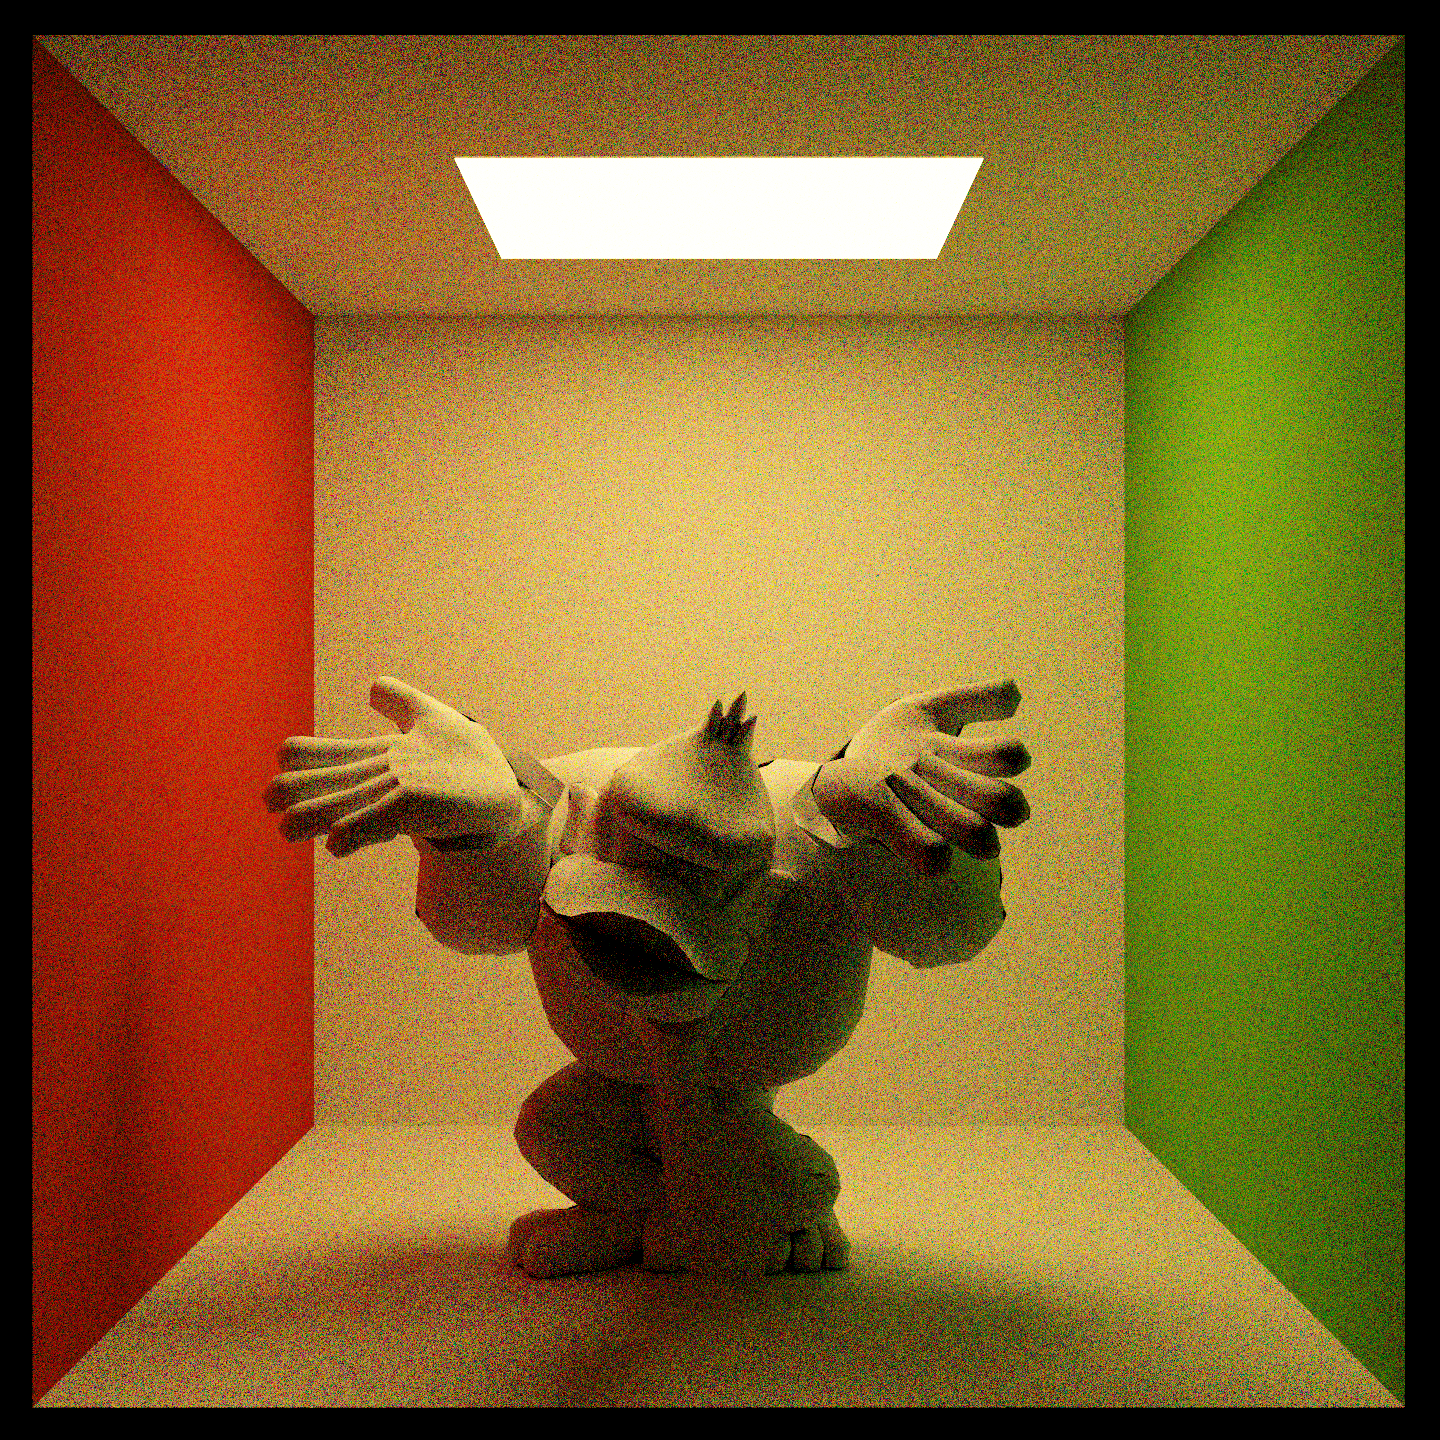
\includegraphics[width=\textwidth]{dk_256spp.png}
        \caption{somethingx4}
        \Description{Image}
        \label{fig:teaser4}
    \end{subfigure}
    \caption{something something}
    \Description{Image}
    \label{fig:teaser}
\end{teaserfigure}

\maketitle

% INTRO
\subfile{chapters/intro1}

% \cite{PBRT4e}

% NEXT SECTION
% \newpage
\nocite{*}
\bibliographystyle{ACM-Reference-Format}
\bibliography{references}
\end{document}